\subsection{Why Use Convolutions?}

So far we understand the building blocks of CNNs and the reasons they are used. The convolution operation is not only used because it is more efficient in image processing, but also because it is inspired by our own visual system.

Like many other neural network topologies, CNNs were bio-inspired by studies on the visual cortex of the human brain that began to take place since 1980 \cite{geron2019}, mainly from the work of David H. Hubel and Torsten Wiesel, where experiments conducted on animals allowed them to deduce the functioning of the structure of the visual cortex.

In short, light signals received by the retina are transmitted to the brain through the optic nerve, where they reach the primary visual cortex, which is mainly formed by two types of cells \cite{goodfellow2016}:

\begin{itemize}
\item \textbf{Simple cells}: these cells have behaviors that can be represented by linear functions in an image with small area known as the receptive field \cite{goodfellow2016,geron2019}. This type of cell inspired the simplest detector units on CNNs.
\item \textbf{Complex cells}: they also respond to features of the image, such as simple cells, but are invariant in position, that is, they do not make much distinction from where the feature appears. This type of cell inspired the pooling units \cite{goodfellow2016}.
\end{itemize}

Anatomically, the deeper we go into the layers of the brain, the more layers analogous to convolution and pooling are used, and we find more specialized cells that respond to specific patterns unaffected by input transformations. Until reaching these deeper layers, a sequence of detections followed by pooling layers is performed \cite{goodfellow2016}. 

\subsection{Classic CNNs}
\label{sec:architectures}

\subsubsection{LeNet} \label{lenet}

After studying the main building blocks of a CNN -- convolutional layers, pooling layers and fully connected layers -- it becomes easier to compare CNNs architectures and we can realize that even with the differences they present a pattern in the combination of layers. Typically, CNN architectures have an interleaved sequence of convolution layer, followed by a pooling layer, which repeats up to the edge of the network where there are some fully connected layers with similar structure to MLP networks. An example of this basic structure was shown in Figure \ref{fig:figure123}. 

Figure \ref{fig:lenet} illustrates a LeNet CNN. As the operations are carried out along this network, it is noticed that the feature maps are getting smaller and that the layers deeper, that is, the number of maps in the same layer increases. As the output layer usually presents itself as a vector of probabilities for each class, there is a transition from the representation of the data in maps to a vector, starting from the flattening process, which occurs before the first fully connected layer.

\begin{figure}[h]
    \centering
    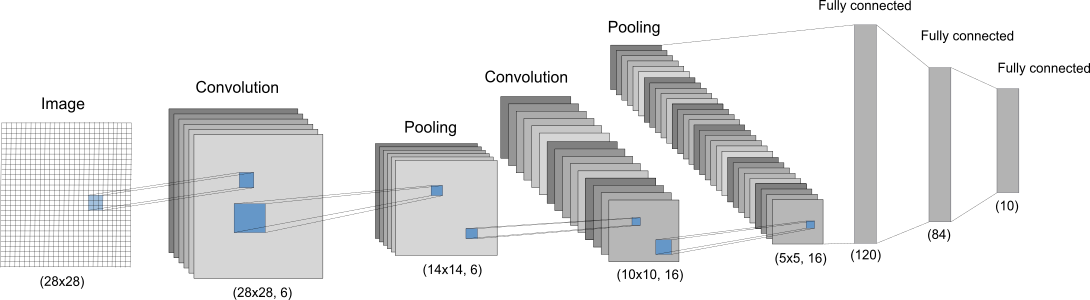
\includegraphics[scale=0.4]{"Part 3 - Learning Systems/Supervised Learning/Deep Learning/images/figure125.png"}
    \caption{ LeNet Convolutional Network - The input is an image of a handwritten number and the output a vector with the probability for each of the ten digits from 0 to 9 \cite{zhang2020dive}.}
    \label{fig:lenet}
\end{figure}

The LeNet network was one of the first CNNs that showed potential application in computer vision. The network was created by Yann LeCun in 1998 for the purpose of handwriting number recognition. LeNet was later adapted to recognize digits for ATM machine deposits, and there are still ATMs that run the code developed by Yann and his colleague Leon Bottou \cite{zhang2020dive}. The network was also widely used for digit recognition of the MNIST dataset \cite{geron2019}. %, this dataset was covered in topic \ref{backpropagation}.

In Figure \ref{fig:lenet}, we take as input a standard MNIST grayscale image, of size 28 x 28 pixels. In the general scheme of the LeNet network (Figure \ref{fig:lenet2}), we have a clearer view of the combination of layers, where after the input layer there are two convolutional layers, each followed by a pooling layer, and at the end there are three fully connected layers.

\begin{figure}
    \centering
    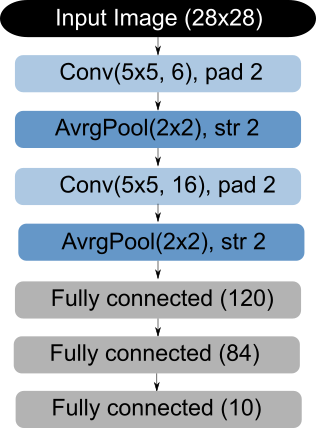
\includegraphics[scale=0.4]{"Part 3 - Learning Systems/Supervised Learning/Deep Learning/images/figure126.png"}
    \caption{ General diagram of layers in the LeNet network - Schematic of the LeNet network with the sequence of convolutional layers (“Conv”), pooling (“AvrgPool”) and fully connected layers \cite{zhang2020dive}.}
    \label{fig:lenet2}
\end{figure}

Each convolution layer uses a filter $5 \times 5$ and a sigmoid activation function (see the chapter about MLPs for a definition of activation functions). The first convolution layer has $6$ channels or maps, while the second one has $16$. The pooling operation involves a filter $2 \times 2$ that calculates the average, so it is identified as “AvrgPool”, and uses stride $str=2$, so that each map from the previous layer is reduced in a half along the width and height, eliminating $75\%$ of the activations. The size of the three fully connected layers are respectively $120$, $84$, and $10$. The last layer, “Fully connected(10)”, corresponds to the possible number of classes, in this case $10$ (digits from $0$ to $10$). The activation function in the last layer is a Gaussian function.

To understand the effects of each layer on the dataset, we present in Table \ref{table:tablelenet} the dimensions of the outputs of each layer. Table \ref{table:tablelenet} shows that from one convolution block to the other there is an increase in the number of channels (C) from 6 to 16, between the pooling layers these values are not changed, as the process only reduces the width (W) and height (H ) of the channels. In fully connected layers, the dimensions are reduced until the size of the number of classes is obtained.

\begin{center}
\begin{table}[]
\begin{tabular}{|l|c|c|c|c|c|}
\hline
\textbf{Layer}    & \textbf{\begin{tabular}[c]{@{}c@{}}Channel\\ (C)\end{tabular}} & \textbf{\begin{tabular}[c]{@{}c@{}}Size\\ (H,W)\end{tabular}} & \textbf{\begin{tabular}[c]{@{}c@{}}Filter\\ (K)\end{tabular}} & \textbf{\begin{tabular}[c]{@{}c@{}}Memory\\ (kB)\end{tabular}} & \textbf{Parameters} \\ \hline
Inputs            & 1                                                            & 28                                                              &                                                             &                                                                &                     \\ \hline
Convolutional 1   & 6                                                            & 28                                                              & 5                                                           & 18                                                             & 156                 \\ \hline
Avrg Pooling 1    & 6                                                            & 14                                                              & 2                                                           & 5                                                              & 0                   \\ \hline
Convolutional 2   & 16                                                           & 10                                                              & 5                                                           & 6                                                              & 2416                \\ \hline
Avrg Pooling 2    & 16                                                           & 5                                                               & 2                                                           & 2                                                              & 0                   \\ \hline
Flatten           & 400                                                          &                                                                 &                                                             & 1.6                                                            & 0                   \\ \hline
Fully Connected 1 & 120                                                          &                                                                 &                                                             & 0.5                                                            & 48120               \\ \hline
Fully Connected 2 & 84                                                           &                                                                 &                                                             & 0.3                                                            & 10164               \\ \hline
Fully Connected 3 & 10                                                           &                                                                 &                                                             & 0.04                                                           & 859                 \\ \hline
Total             &                                                              &                                                                 &                                                             & 33                                                             & 61706               \\ \hline
\end{tabular}
\caption{LeNet Layer Settings, Parameters and Information - Summary of LeNet's main layer settings such as number of channels and filter size. Display an estimate of the number of parameters and the amount of memory to train the network.}

\label{table:tablelenet}
\end{table}
\end{center}

It is common in CNN's networks that the number of channels practically doubles after a pooling layer since there is a reduction by half in the dimensions of the maps. Thus, it is possible to increase the number of maps, making it more sensitive to identify low-level features such as borders and textures, without drastically increasing the number of parameters and computational resources \cite{zhang2020dive}. As the first convolution layer applies  $\text{padding}=2$, the maps maintain the same dimension in the output as the original image ($28 \times  28$), however the second layer does not have padding, which reduces the width and height of the maps by $4$ pixels.

Over the years, variations of this model have emerged and the most evident difference between the networks is the number of layers, which has increased over the years, making the networks deeper. When increasing the number of layers it was noticed that the performance of the networks tended to improve, however some limitations emerged. The greater the amount of data, the more computational memory is required, and this capacity depends on hardware requirements.

To assess the amount of memory used in training the LeNet network, we will use an approximate calculation based on the amount of output elements in each layer. The number of elements is multiplied by the number of bytes needed to store each element \cite{johnson2019}. Considering that floating point data occupy $32 \text{ bits}$, therefore  $4 \text{ bytes}$ per element, to facilitate the visualization of the results, the measure kilobyte (kB) is used, and for this reason they were divided by the factor 1024 since  $1 \text{ kB} = 1024 \text{ B}$ . In Equation \ref{qtdMemoria}, we exemplify the calculation of the amount of memory for the first convolution layer of the LeNet network:


\begin{equation}
\begin{split}
\text{Amount of memory }& = \text{CxHxW}\\ 
&= 6 \times  28 \times  28\\
&= 4704 \text{ output elements}\\
&= 4704 \times 4 \text{ bytes} = 18816 \text{ bytes}\\
&= 18.38 \text{ kilobytes}
\end{split}
\label{qtdMemoria}
\end{equation}

The C parameter identifies the number of channels or maps of the layer and the term H and W, the height and width of the layers output element, respectively. As shown in Equation \ref{qtdMemoria} and Table \ref{table:tablelenet}, the approximate amount of memory for the first layer is $18 \text{ kB}$, and in total for the network $33 \text{ kB}$. The first layers tend to need more memory due to the larger dimensions (W and H) of the channels \cite{johnson2019}.

Increasing the number of layers also requires that more parameters be learned, which affects both the training time and its performance, because if there is not an adequate optimization of the parameters, the probability of overfitting can be higher \cite{elgendy2020}. To approximately determine the number of parameters related to each layer, the weights related to the filters of each map were considered, calculated as the product between the filter dimensions ($\text{K x K}$), the number of input element channels and the number of output channels of the layer \cite{johnson2019}. The biases associated to each output channel were also considered as parameters. On fully connected layers, the number of parameters is determined as the product of the number of input elements and the number of output elements of the layer plus the number of biases. Equation \ref{calcConvInfos} exemplifies the calculations for the first convolution layer:

\begin{equation}
\begin{split}
  \text{Weights} &= \text{C}_\text{output} \times  \text{C}_\text{input} \times  \text{K} \times  \text{K}\\ 
  &= 6\times 1 \times  5 \times  5\\
  &= 150\\\\
  \text{Bias} &= 6\\\\
  \text{Parameters} &= \text{Weights} + \text{Bias}\\
  &= 150 + 6\\
  &= 156
\end{split}
\label{calcConvInfos}
\end{equation}

Considering that the filter in the first layer is of size $5\times 5$, that the input has only 1 channel and that there are 6 channels in the convolution layer, the first convolution layer considers approximately 156 parameters. In Table \ref{table:tablelenet}, there is also the number of parameters related to each layer and the approximate total of parameters for the LeNet network is 61706. As the number of channels in the convolution layer increases, more parameters are needed. In general, most parameters are due to fully connected layers due to the greater number of connections \cite{johnson2019}.

\subsubsection{AlexNet}

Currently there are several CNNs network architectures used for applications in computer vision. The evolution of these networks can be seen in the results of the ImageNet Large Scale Visual Recognition Challenge (ILSVRC) competition. The main objective of the competition was to evaluate algorithms for object detection and image classification. The first edition of the competition, in 2010, involved 1.2 million images for training, being 1000 categories of objects. In the first two years of competition, CNNs networks weren't yet in 1st place, however, from on 2012 CNNs models started to lead the competition \cite{imagenet2020}. The progress of the networks can be evaluated based on the error rate of the models, which in seven years dropped from approximately $26\%$, in the second year of the competition, to $2.3\%$ in the last edition of the competition in 2017 \cite{johnson2019}, as shown in the graph in Figure \ref{fig:imagenet}.


\begin{figure}
    \centering
    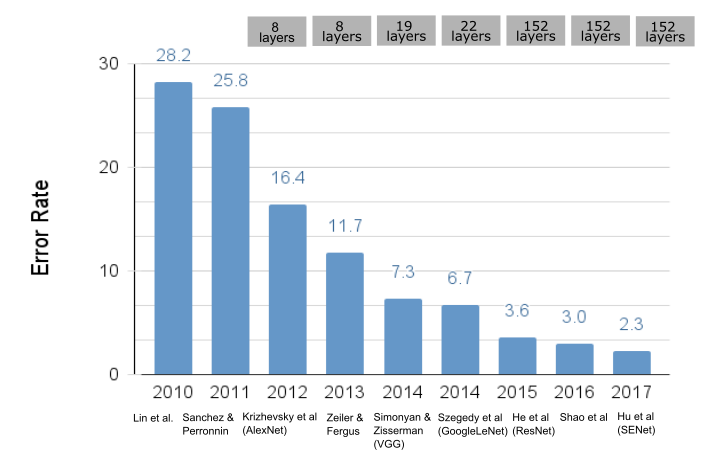
\includegraphics[scale=0.4]{"Part 3 - Learning Systems/Supervised Learning/Deep Learning/images/figure127.png"}
    \caption{ Error rate of the best performing models in the ImageNet competition - The performance of the models in the ImageNet Large Scale Visual Recognition Challenge (ILSVRC) competition was mainly evaluated by the error rate. The graph shows the models that won in each edition of the competition, which ran from 2010 to 2017, and also networks that became popular such as VGG \cite{johnson2019}.}
    \label{fig:imagenet}
\end{figure}

To learn a little about the different architectures of CNNs networks and notice some differences, and structures that performed well and are still adopted by recent architectures, we will highlight below three additional architectures that become well known and had prominence in the competition. The AlexNet network was the first CNN to win the ImageNet competition in 2012 with an error rate of $16.4\%$. The VGG network did not lead the competition in 2014, but it is one of the models with great popularity. In 2014, the CNN GoogLeNet won the competition and served as inspiration for the Inceptions networks. %The Residual network (ResNet) in 2015, in addition to taking advantage of the higher performance techniques of other networks, also carried an approach that made it possible to increase its depth to more than 100 layers.

The AlexNet network was developed by Alex Krizhevsky, Ilya Sutskever, and Geoffrey Hinton \cite{geron2019}. This network is very similar to LeNet, but has more layers. Because it is a deeper network, requiring more memory, the original network had to be physically distributed between two 3GB GPUs  \cite{krizhevsky2012}. In this way, the network was drawn as in Figure \ref{fig:alexnet}, with a dual data stream structure so that each GPU would receive half of the model.

\begin{sidewaysfigure}[p]
    \centering
    \vspace{10cm}
    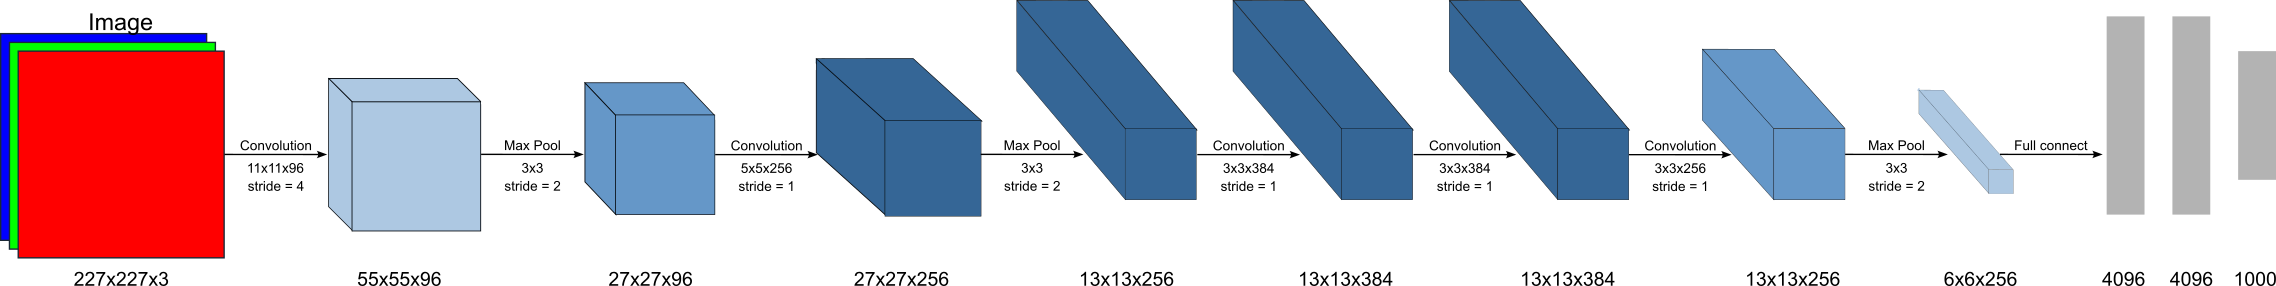
\includegraphics[scale=0.4]{"Part 3 - Learning Systems/Supervised Learning/Deep Learning/images/figure128.png"}
    \caption{ AlexNet network architecture - represented as the combination of two identical networks, as originally the training would occur with the distribution of data between two GPU's \cite{krizhevsky2012}.}
    \label{fig:alexnet}
\end{sidewaysfigure}

As depicted in Figure \ref{fig:lenetalexnet}, AlexNet has 5 convolution layers, with the first three followed by pooling layers. The most aparent difference between the AlexNet and LeNet architectures are the three additional convolution layers in the AlexNet network, which are followed one after the other with no layer pooling between them. As the input images are bigger than the MNIST dataset approached in the example LeNet network, the input convolution filters are bigger ($11\times 11$) and stride $\text{str} = 4$ is used. In the second convolution layer, the filters have size $5\times 5$, and in the other convolution layers filters $3\times 3$ are used.

With the discovery that ReLU's activation functions in the convolution layers and that maxpooling improve the performance of networks, most models were built using these functions \cite{zhang2020dive}. Maxpooling filters of size $3\times 3$ and stride $\text{str} = 2$ scale down channels based on the largest value of the receive field. With the exception of the first layer, all other convolution layers are padded so that the dimension of the channels is not changed after the convolutions.

The last three layers are fully connected and have sizes 4096, 4096 and 1000, respectively. The output layer has dimension 1000 due to the number of possible classes of ImageNet competition and the activation function is Softmax.

\begin{figure}[h]
    \centering
    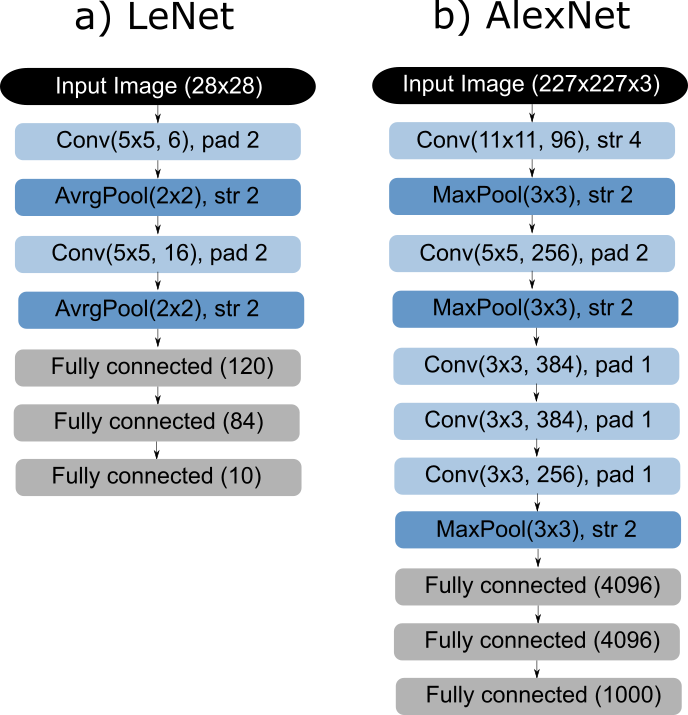
\includegraphics[scale=0.4]{"Part 3 - Learning Systems/Supervised Learning/Deep Learning/images/figure129.png"}
    \caption{ Comparison of AlexNet and LeNet networks. (a) LeNet Network and (b)  AlexNet Network. These general layer schemes show that the main difference of networks is that AlexNet is deeper, with three more convolution layers than LeNet \cite{zhang2020dive}.}
    \label{fig:lenetalexnet}
\end{figure}

The same pattern for the dimensions of the layer output elements seen in LeNet is seen in Table \ref{table:tablealexnet} for the AlexNet network. While the size of the channels decreases from one convolution layer to another, the number of channels increases, with 96 in the first, followed by 256, 384, 384 and 256. After the flatten process, the dimension of the layers is reduced until it is established the size of the prediction classes vector.

By comparing the amount of memory and the approximate number of parameters as described in the subsection \ref{lenet} it is observed that the amount of memory required increases and the number of parameters also increases. Approximate calculations indicate that while the memory required for training the LeNet network would be approximately $33 \text{ kB}$, for AlexNet it would be approximately $3\text{ GB}$. The number of parameters calculated for LeNet was 62 thousand and for AlexNet 62 million.  Generally in both models, the first layers require more memory, while the fully connected layers need more parameters.

\begin{center}
\begin{table}[]
\begin{tabular}{|l|c|c|c|c|c|}
\hline
\textbf{Layer}    & \textbf{\begin{tabular}[c]{@{}c@{}}Channel\\ (C)\end{tabular}} & \textbf{\begin{tabular}[c]{@{}c@{}}Size\\ (H,W)\end{tabular}} & \textbf{\begin{tabular}[c]{@{}c@{}}Filter\\ (K)\end{tabular}} & \textbf{\begin{tabular}[c]{@{}c@{}}Memory\\ (kB)\end{tabular}} & \textbf{Parameters} \\ \hline
Inputs            & 3                                                              & 227                                                           &                                                               &                                                                &                     \\ \hline
Convolutional 1   & 96                                                             & 55                                                            & 11                                                            & 1134                                                           & 35                  \\ \hline
Max Pooling 1     & 96                                                             & 27                                                            & 3                                                             & 273                                                            & 0                   \\ \hline
Convolutional 2   & 256                                                            & 27                                                            & 5                                                             & 729                                                            & 615                 \\ \hline
Max Pooling 2     & 256                                                            & 13                                                            & 3                                                             & 169                                                            & 0                   \\ \hline
Convolutional 3   & 384                                                            & 13                                                            & 3                                                             & 254                                                            & 885                 \\ \hline
Convolutional 4   & 384                                                            & 13                                                            & 3                                                             & 254                                                            & 1327                \\ \hline
Convolutional 5   & 256                                                            & 13                                                            & 3                                                             & 169                                                            & 885                 \\ \hline
Max Pooling 3     & 256                                                            & 6                                                             & 3                                                             & 36                                                             & 0                   \\ \hline
Flatten           & 9216                                                           &                                                               &                                                               & 36                                                             & 0                   \\ \hline
Fully Connected 1 & 4096                                                           &                                                               &                                                               & 16                                                             & 37753               \\ \hline
Fully Connected 2 & 4096                                                           &                                                               &                                                               & 16                                                             & 16781               \\ \hline
Fully Connected 3 & 1000                                                           &                                                               &                                                               & 4                                                              & 4097                \\ \hline
Total             &                                                                &                                                               &                                                               & 3090                                                           & 62378               \\ \hline
\end{tabular}
\caption{AlexNet Layer Settings, Parameters, and Information - Summary of settings for the main AlexNet layers, such as number of channels and size of filters. Display an estimate of the number of parameters and the amount of memory to train the network.}

\label{table:tablealexnet}
\end{table}
\end{center}

\subsubsection{VGG} \label{vgg}

The VGG network was conceived by the members of the Visual Geometry Group (VGG) at Oxford University by researchers Karen Simonyan and Andrew Zisserman \cite{zhang2020dive}. Compared to the two previous architectures LeNet and AlexNet, VGG adopts principles to establish the structure of the network, which allowed the construction of deeper models \cite{zhang2020dive}. Another characteristic of VGG is the block structure in the part of the network with the convolutional layers, in which each block presents convolutional layers in sequence and at the end a pooling layer. While the AlexNet model, in Figure \ref{fig:alexnetvgg}, presents 5 convolutional layers, the VGG presents 5 blocks with a variable number of convolution layers, but in general the first blocks have fewer layers. Like AlexNet, at the edge of the network there are three fully connected layers, with equal dimensions on both models, and a Softmax activation function at the output.

In Figure \ref{fig:alexnetvgg}, there is a representation of the VGG architecture with 16 layers, in which the first two blocks have two convolutional layers and the last three blocks have three convolutional layers. The convolution layers double in size with each block, with each layer in the first block having 64 channels, 128 channels in the next, and so on up to 512 in the last block. The use of the ReLu activation function in the convolution layer and maximum value pooling are strategies that performed well in AlexNet and continued in other models, such as in VGG.

\begin{figure}[h]
    \centering
    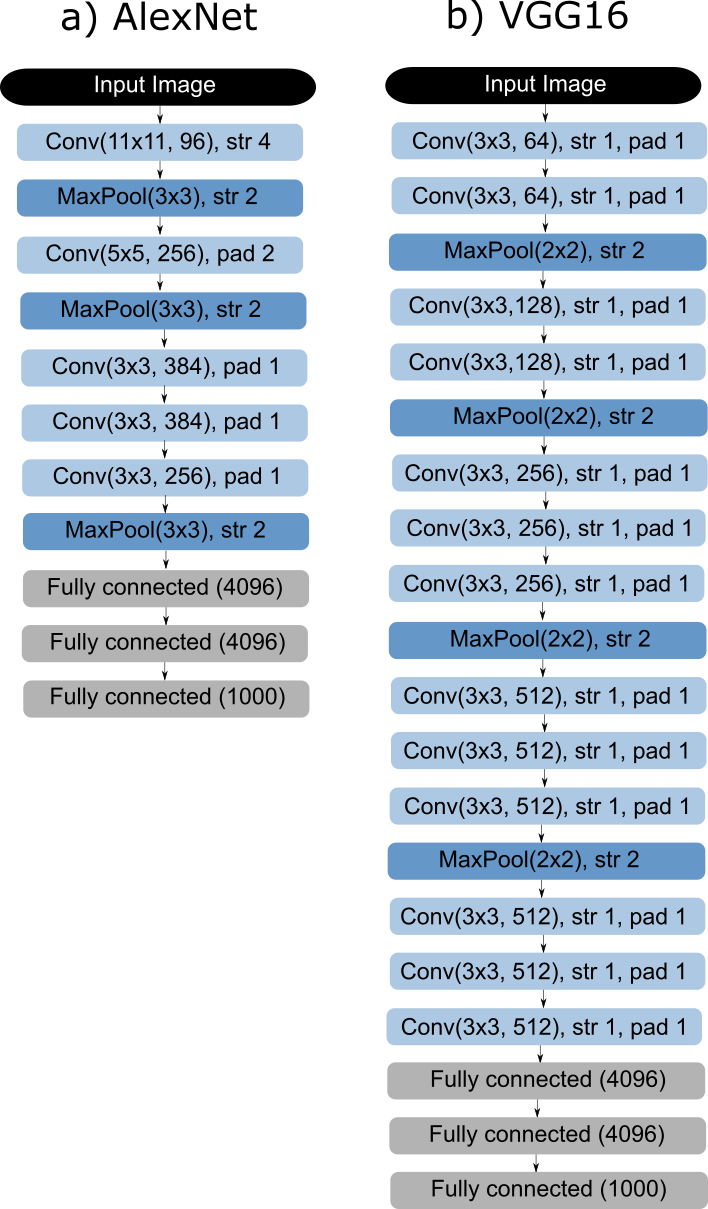
\includegraphics[scale=0.4]{"Part 3 - Learning Systems/Supervised Learning/Deep Learning/images/figure130.png"}
    \caption{ Comparison of VGG and AlexNet networks - Comparison of VGG and AlexNet networks based on the general structure of the layers. While the final part of the networks is similar in relation to the fully connected layers, the VGG differs in that it is deeper and presents a pattern of convolutional layers organized in blocks  \cite{johnson2019}.}
    \label{fig:alexnetvgg}
\end{figure}

In LeNet and AlexNet networks, it is usually necessary to individually select several hyperparameters\footnote{Hyperparameters are parameters that need to be pre-defined, as opposed to learned by the model.}. For example, in the convolution layers, the number of channels, size of filters, padding and stride are adjustable. In the pooling layer, the hyperparameters are the filter and stride size. In general, these two networks do not provide a general guide on how to select the parameters. VGG's core design principles state that all convolution filters are $3\times 3$ with stride $\text{str} = 1$ and padding $\text{pad} = 1$, and that maxpooling filters are $2\times 2$ with $\text{str} = 2$. After each pooling layer, the number of channels doubles in the convolution layer. The idea of fixing the size of convolutional filters came from the perception that the combination of two filters $3\times 3$ presents a receptive field equivalent to one filter $5\times 5$, and that three filters $3\times 3$ perform similar to one of $7\times 7$ \cite{elgendy2020}. Fixing the size of filters and their stride $\text{str} = 1$ and $\text{pad} = 1$ establishes that the dimension of the channels does not change between the convolutional layers, so the only hyperparameter that needs to be optimized is the number of layers in each block.

By using filters $3\times 3$, which are smaller, but in greater quantity than those used in AlexNet ($11\times 11$ and $5\times 5$), more nonlinearity is included, allowing the network to learn more low-level features \cite{elgendy2020}. Increasing the depth of the network with more layers of convolution adds more non-linear activation functions. Even being deeper networks, this strategy of using smaller filters reduces the number of parameters. Considering that two layers in sequence have C channels each, when using two filters $3\times 3$, the total number of parameters is $2\times 3\times 3\times \text{C}^2 = 18\text{C}^2$, which is smaller number when compared to the scenario of a single filter $5\times 5$ with $25\text{C}^2$ parameters \cite{johnson2019}.

Of course, doubling the number of channels between blocks should make the number of parameters grow quickly, and that's why maxpooling filters have been standardized to reduce the dimensions of the channels by half. By controlling the number of activations that pass to the next layers, it is possible to keep the number of operations approximately constant. Superficially evaluating that the number of operations is given as the total amount of multiplications and additions, we can calculate for each layer as the product of four parameters in Equation \ref{numOperacoes} \cite{johnson2019}: filter size($\text{K x K}$), input channel dimensions ($\text{H x W}$), quantity of input channels ($\text{C}_{\text{input}}$) and output channels ($\text{C}_{\text{output}}$).

\begin{equation}
\begin{split}
  \text{Number of operations} &= \text{Number of output elements x Operations by output element}\\
  &= (\text{C}_{\text{output}} \text{ x H x W}) \times  (\text{C}_{\text{input}} \text{ x K x K})\\
  &= (2\text{C x HW}) \times  (\text{2C x 3 x 3})\\
  &= 36 \text{HWC}^2
\end{split}
\label{numOperacoes}
\end{equation}

In the case of two convolution layers with filters $3\times 3$ and separated by a pooling, reducing by half the size of the channels ($\text{2H x 2W} \rightarrow \text{H x W}$) and doubling the number of channels ($\text{C} \rightarrow \text{2C}$), the number of weights increases from $9\text{C}^2$ to $36\text{C}^2$, but the number of operations remains at $36\text{HWC}^2$.

\subsubsection{GoogLenet and Inception} \label{inception}

By following the evolution of CNNs, we can see that the main strategy to increase the performance in the classification of images was to increase the number of layers that keep the weights of the networks. AlexNet and VGG-16 networks were developed with 8 and 16 layers, respectively. As the networks get deeper, the dilemma of how to make the algorithms more efficient arose, since more layers meant more parameters and operations, requiring more computational resources. Comparing the networks in Figure \ref{fig:neuralevolution}, it is possible to verify the accuracy of the networks, the number of parameters and the number of operations. It appears that for the VGG-16 network to achieve better results than the AlexNet network, it was necessary to more than twice the number of parameters, from approximately 65 million on AlexNet to just over 130 million on VGG-16.

In the 2014 ImageNet competition, a Google research group led by Christian Szegedy proposed the GoogLeNet architecture that should both ensure good performance and be more efficient than existing models \cite{geron2019}. The model not only won the competition but also met their requirements, as even being a network with 22 layers, more than the VGG-16, it used 12 times less parameters than VGG, 13 million instead of 138 million \cite{elgendy2020}.

\begin{figure}
    \centering
    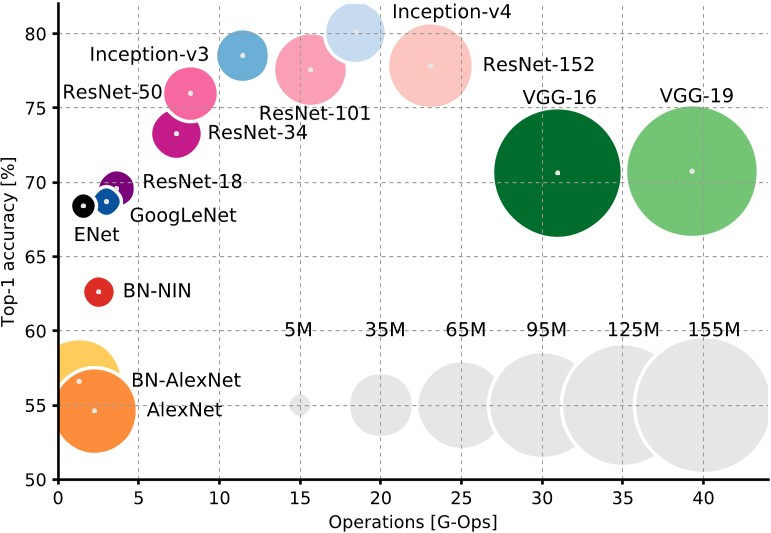
\includegraphics[scale=0.4]{"Part 3 - Learning Systems/Supervised Learning/Deep Learning/images/figure131.jpg"}
    \caption{ CNN's neural networks evolution graph - Network performance is evaluated by accuracy versus the number of operations required for a single forward step. The radius of the circles is proportional to the number of parameters, with the legend in the lower right corner indicating a reference from $5\times 10^6$ to $155\times 10^6$ \cite{canziani2016}.}
    \label{fig:neuralevolution}
\end{figure}

To understand the GoogLenet network we can divide it into three parts (Figure \ref{fig:googlenet}), in the first part, the input layers are similar to the AlexNet and VGG networks, in the second part, there are the inception blocks characteristic of this network, and the last part refers to the classification structure. The first part contains two blocks with a sequence of convolutional layers followed by pooling $3\times 3$. In the first block, there is only a convolution layer $7\times 7$, with stride $\text{str} = 2$ and padding $\text{pad}= 3$, and a pooling layer with $\text{str} = 2$. At the end of these two layers, the element has 64 channels and was reduced by 4 in its dimension (H and W). In the second block, there are two convolution layers, the first with a filter $1\times 1$ and 64 channels and the second $3\times 3$ with 192 channels, and only the pooling $3\times 3$ at the end of the block changes the dimensions of the channels in half.

The main role of these two blocks is to reduce considerably the dimensions of the image, since most of the memory required is due to the first layers \cite{johnson2019}. Whereas, at this stage, there is an 8-fold reduction in image dimensions, an entry $224\times 224$ when reducing to approximately $28\times 28$ use approximately $7.5 \text{ MB}$ memory while the same reduction in VGG-16 needs $42.9 \text{ MB}$, almost $6$ times more than GoogLenet \cite{johnson2019}. Also, when passing a smaller image to the next layers, the number of operations and the number of parameters to train the network are also reduced.

\begin{figure}
    \centering
    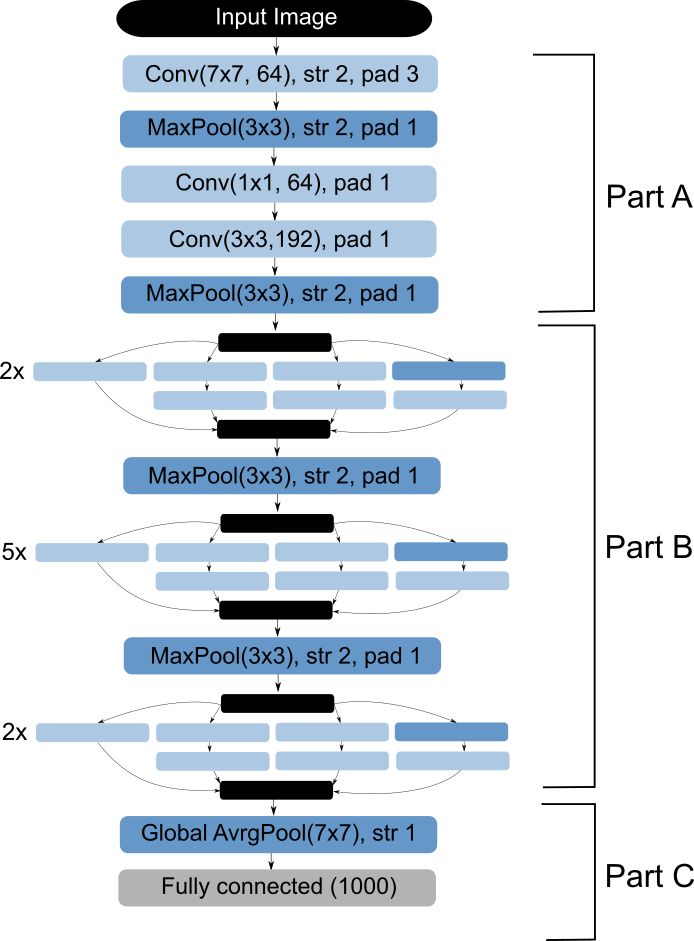
\includegraphics[scale=0.4]{"Part 3 - Learning Systems/Supervised Learning/Deep Learning/images/figure132.png"}
    \caption{ The general structure of the GoogLenet network can be divided into three parts: Part A - Similar to AlexNet and LeNet, contains a sequence of convolutional layers and pooling to reduce image dimensions; Part B - Inceptions modules separated by pooling layers; Part C - Global pooling layer and a Fully Connected for classification \cite{elgendy2020}.}
    \label{fig:googlenet}
\end{figure}

Another technique to make the network more efficient was to include a global AvrgPool layer before the classification layer \cite{geron2019}. In previous CNN models it was common to include flattening to convert the data into a vector, losing the spatial information, to be compatible with the fully connected layers that made the classification. These last layers end up being responsible for most of the parameters. In the VGG-16 model, for example, the 3 fully connected layers generate approximately $123.6$ millions of parameters, almost $90\%$ of the total parameters \cite{johnson2019}.

Instead of adopting flattening, GoogLenet uses an averaging filter of the same dimension as the input element, returning the average of the maps for each position of the vector. As the output vector is already reduced in size, it is necessary to include only one layer fully connected with $1000$ classes. Since the global averaging layer does not need parameters, and since it returns a vector $1024$, approximately $1$ million parameters are needed in the fully connected layer, $100$ times less than in the VGG \cite{johnson2019}. In the last layer, as in the VGG, a Softmax activation is associated, while in the convolution layers it is a ReLu.

The first and last parts of the GoogLenet network have been explained above. The intermediate section that we will study now includes the Inceptions modules that have become characteristic elements of the most modern networks. Each module is similar to VGG blocks, in that some convolutional layers are present in sequence and at the end a pooling layer. In the case of the VGG, it was seen that to reduce the number of hyperparameters, the size of the filters was set to $3\times 3$, and the variable parameter was the number of convolutional layers. The idea of Inceptions (Figure \ref{fig:inceptionmodule}) is not to worry about the size of the filters or the number of layers in the module, as each module consists of a combination of filters with different sizes arranged in a fixed way \cite{elgendy2020}.

\begin{figure}
    \centering
    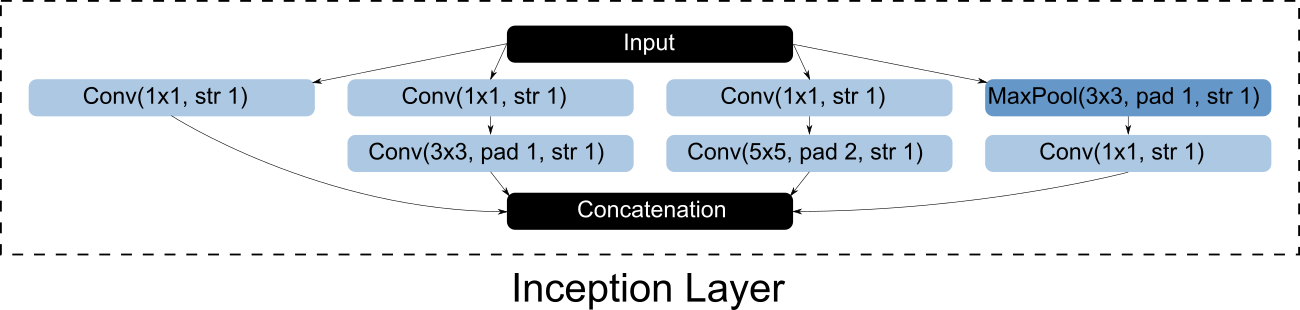
\includegraphics[scale=0.34]{"Part 3 - Learning Systems/Supervised Learning/Deep Learning/images/figure133.png"}
    \caption{ Inception module of the GoogLenet network - The middle part of the GoogLenet network is formed by a sequence of Inceptions modules separated by pooling layers (Figure \ref{fig:googlenet}). Each module has four paths to the same input data, and on output, where the results are concatenated \cite{zhang2020dive}.}
    \label{fig:inceptionmodule}
\end{figure}

From the input of the inception module, copies of the input element go along four paths at the same time. At the end of these paths, the image size does not change, but the number of channels is changed in different ways, with the choice of the number of channels for each layer being a hyperparameter. At the output of the module there is a concatenation of all these channels, forming a single element with the same dimension as at the input and with a number of channels that is the sum of all that resulted from each path.

The first path has only one convolution $1\times 1$, known as the bottleneck, whose main function is to preserve the dimensions (height and width) but reduce the number of channels, which reduces the computational cost and the number of parameters \cite{elgendy2020}. As this convolution includes more nonlinearity at a low cost, a convolution $1\times 1$ is also included in the input layers, contributing to an optimization in the first part of the network \cite{geron2019}. This same layer has been added at the beginning of each of paths 2 and 3 to reduce model complexity. After reducing the number of layers, larger filters are included, making it possible to process information at different scales, with the filters being in the second way $3\times 3$ and in the fourth way  $5\times 5$ \cite{zhang2020dive}.

All paths, even the fourth that includes a MaxPool layer, feature padding to keep the same dimension of the channels as in the entrance. As MaxPool does not change the number of channels, a convolution $1\times 1$ is included at the end of the fourth path, reducing the volume.

By concatenating all the channels of each path at the end, the inception module follows the hypothesis that visual information can be processed at various scales and that the aggregated results allow the next level to extract several features from different scales at the same time \cite{elgendy2020}. In the GoogLenet network in Figure \ref{fig:googlenet}, we see three groups of inception modules interspersed by Maxpooling $3\times 3$, totalling 9 modules.

The previous GoogLenet diagram (Figure \ref{fig:googlenet}) is one of the more simplified representations of the model, because as seen in Figure \ref{fig:googlenet2}, the original architecture includes two classifiers that run in parallel with the other blocks described above, one that starts after the third inception module and the other after the sixth module \cite{geron2019}. Each classifier works similarly to the final part of the network, where classification takes place \cite{johnson2019}. The classifiers are formed by an AvrgPooling layer, followed by a convolution layer, two fully connected layers and at the output a Softmax activation function.

\begin{figure}
    \centering
    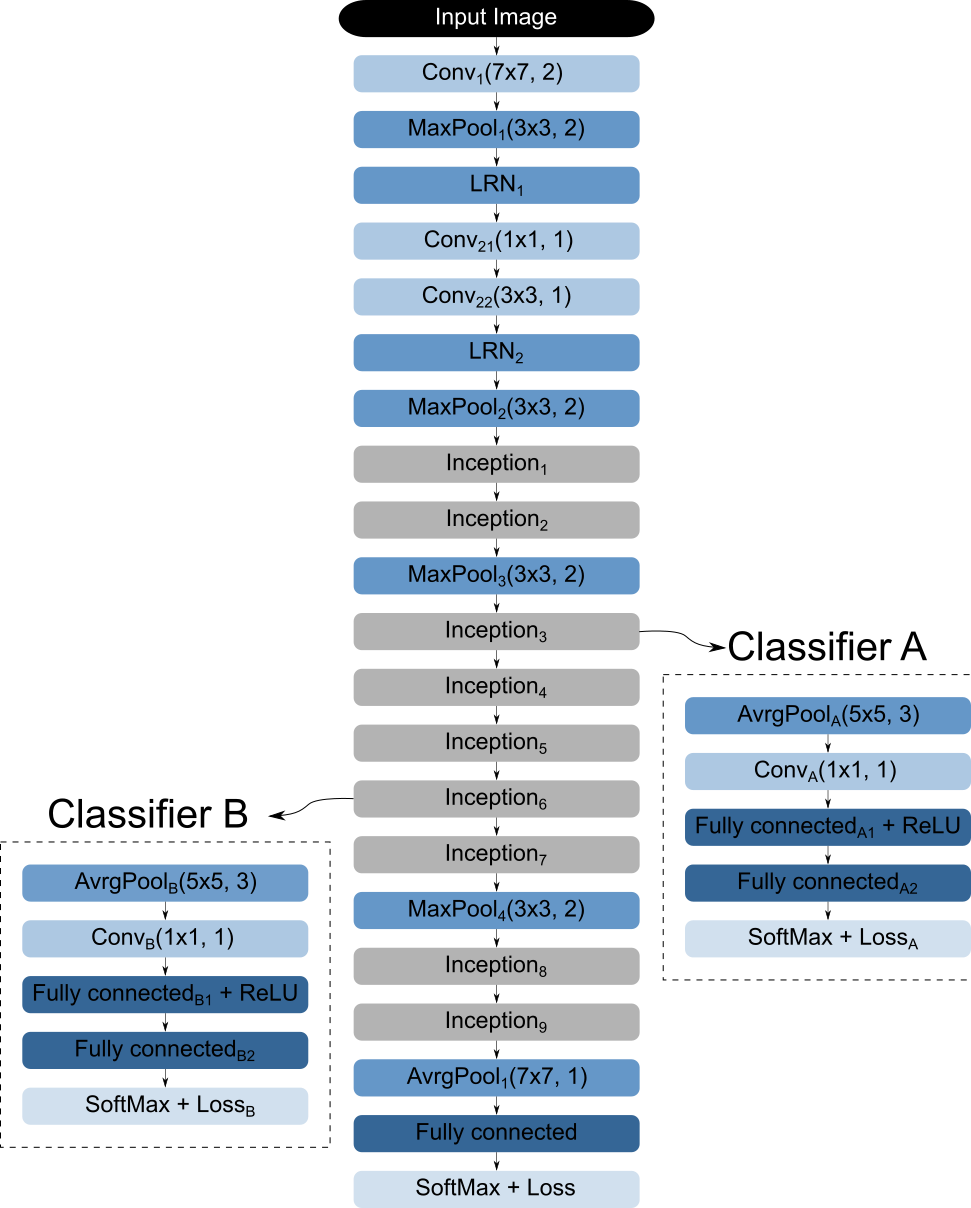
\includegraphics[scale=0.4]{"Part 3 - Learning Systems/Supervised Learning/Deep Learning/images/figure134.png"}
    \caption{GoogLenet network architecture with intermediate classifiers - The GoogLenet network with two classifiers, one in the third inception module and the other in the sixth module. These intermediate classifiers reduce the fading effect of error gradients \cite{img:googlenet}.}
    \label{fig:googlenet2}
\end{figure}


There is a peculiarity when training deeper networks, because, in the backpropagation of errors, the rates reduce to values very close to zero, making it difficult for the algorithm to converge. One of the techniques adopted by GoogLenet to help convergence was to include the calculation of the error gradient of these intermediate classifications in the error backpropagation \cite{geron2019}.

